\section{Desarrollo}

Para alcanzar los objetivos planteados en la introducción, vamos a proponer distintos análisis, organizados según el orden cronológico de
la investigación. Un detalle importante a destacar es que basaremos todo el análisis en la version 4 del protocolo de internet, con lo cual
cada vez que se mencionen direcciones IPs o características del protocolo IP, siempre nos referiremos la version 4\cite{internetprotocolv4}.

\subsection{Determinación de rutas entre dos hosts} \label{desarrollo:rutas}
Antes de poder realizar ningún tipo de estimación, debemos encontrar la/s ruta/s entre dos hosts: fuente ($H_{src}$) y destino ($H_{dst}$). Para
esto utilizaremos una de las técnicas de traceroute.

El encabezado de un paquete IP\cite{internetprotocolv4} tiene un campo de 8 bits llamado TTL (Time To Live) que indica la máxima cantidad de segundos
que el paquete IP puede permanecer en la internetwork. Dado que cuando un paquete pasa por un router generalmente tarda menos de un segundo,
el TTL es decrementado de todas maneras (porque si no nunca sería decrementado y no serviría de nada), con lo cual en la realidad el
\emph{TTL indica la cantidad máxima de saltos} que el paquete puede realizar antes de ser descartado.

Cuando un paquete IP llega a un nodo con TTL=$t$, a menos que fuera el host destino, lo decrementa y forwardea el paquete con TTL=$t-1$.
Si al decrementarlo sucede que $t-1=0$, el paquete es descartado y \emph{no se forwardea}. Además el nodo tiene la opción de enviar al host
fuente un paquete IP-ICMP de tipo time-exceeded (TIME-EXC) que indica que el TTL llegó a cero y que el paquete no fue entregado al destino.
La IP fuente de ese paquete es la IP del nodo en la interfaz que recibió el paquete original.

\begin{itemize}
 \item[] Entonces, para determinar una ruta, enviaremos varios paquetes IP aumentando el TTL desde 1,
 para ir recibiendo los TIME-EXC de cada nodo en el camino.
La IP asociada a cada TTL corresponderá a la interfaz por la que ingresó nuestro paquete a ese nodo.
\end{itemize}

Para saber que llegamos a destino, vamos a agregar a nuestro paquete IP un paquete ICMP de tipo ECHO-REQUEST: Si llegamos a destino, es probable
que recibamos una respuesta ICMP de tipo ECHO-REPLY (podría pasar que no la recibieramos, pero para el resto del análisis vamos a elegir destinos
que efectivamente respondan).

\begin{itemize}
 \item[] Entonces el análisis de una ruta finaliza cuando recibimos un paquete ECHO-REPLY (en vez de TIME-EXC).\footnote{En realidad
 seguiremos aumentando el TTL hasta que haya una cierta cantidad de respuestas ECHO-REPLY, y así asegurarnos que no estemos perdiendo una
 ruta alternativa de distinta longitud.}
\end{itemize}

Este análisis lo vamos a repetir muchas veces: Realizaremos $N$ iteraciones de todo este proceso, guardando por cada TTL la IP que respondió, el tipo
de ICMP recibido y el tiempo que transcurrió desde que el paquete fue enviado hasta que se recibió la respuesta. Ese tiempo mide el RTT desde el
host fuente hasta cada uno de los nodos intermedios, con lo cual lo llamaremos $RTT^{acum}_i$ (acumulado para el salto $i$).

Uno de los objetivos de realizar las iteraciones es \emph{encontrar rutas alternativas}. Esto tiene un problema. Supongamos que para $ttl_1$ encontramos
$ip_1$ e $ip_2$, y para $ttl_2$ encontramos $ip_3$ e $ip_4$, y supongamos que $ttl_1 + 1 = ttl_2$. Con esa información, podemos determinar que estos
son los posibles saltos:
\begin{itemize}
 \item $ip_1 \longrightarrow ip_3$
 \item $ip_1 \longrightarrow ip_4$
 \item $ip_2 \longrightarrow ip_3$
 \item $ip_2 \longrightarrow ip_4$
\end{itemize}
No necesariamente son todos válidos. Entonces vamos a contar cuantas veces
respondió cada una de esas IPs y vamos a estimar la probabilidad de pasar por cada nodo en un salto dado (TTL fijo): $P(ip|ttl)$. Usando esas
estimaciones, vamos a ordenar a las IPs según la probabilidad de aparecer en cada salto, y armar los caminos según esas probablidades. En el ejemplo,
supongamos que $P(ip_1|ttl_1) > P(ip_2|ttl_1)$ y $P(ip_3|ttl_2) > P(ip_4|ttl_2)$. Luego los saltos que creemos que serán correctos son:
\begin{itemize}
 \item $ip_1 \longrightarrow ip_3$
 \item $ip_2 \longrightarrow ip_4$
\end{itemize}
Este análisis a priori podría fallar pero insistimos en que es tan sólo una estimación dado que es imposible conocer los enlaces físicos
reales (a menos que controlemos la red).

De todos los caminos que encontremos, elegiremos el más ``pesado'', es decir el camino formado por las IPs con la mayor probabilidad de cada salto.
Para este camino realizaremos los estudios de tiempos y geolocalización.

Otra de las razones por la cual realizamos $N$ iteraciones es para poder estimar $RTT^{acum}_i$ de cada salto. Como dijimos en la introducción, los
RTTs a nivel de red son muy variables y difíciles de estimar (dado que dependen de cada red y de los tiempos de encolamiento de los routers), con lo cual
necesitamos tomar muchas mediciones para poder promediarlas (de alguna manera).

Para este trabajo se eligió $N=1000$, dado que nos pareció una cantidad suficiente para detectar posibles alteraciones en las rutas (por downtime de
un nodo, por congestión, etc). Tener en cuenta que $1000$ iteraciones en Internet corresponden a varias horas de medición.







\subsection{Cálculo del RTT aproximado de cada salto} \label{desarrollo:rttPorSalto}
Como mencionamos en la sección previa, sólo calcularemos el RTT de cada salto en el camino más ``pesado'', de entre todos los caminos posibles.
Hasta ahora tenemos muchos $RRT^{acum}_{ij}$, donde $i$ corresponde al valor de TTL y $j$ a la iteración.
Primero tenemos que quedarnos con un único RTT acumulado para cada salto $i$. Entonces vamos a promediar
de la siguiente manera.

\begin{itemize}
 \item[] Sean $\{RTT^{acum}_{i1}, \dots, RTT^{acum}_{im}\}$ los RTTs acumulados para cada paquete recibido de la IP elegida en el salto $i$.
 Supongamos que están ordenados de manera tal que:
 $$RTT^{acum}_{i1}\leq \dots \leq RTT^{acum}_{im}$$
 Dado un valor $0\leq \alpha < 50$, elminaremos el $\alpha \%$ de los valores más chicos y el $\alpha \%$ de los valores más grandes. Supongamos
 que nos queda:
 $$\{RTT^{acum}_{ia}, \dots, RTT^{acum}_{ib}\}$$
 Luego calcularemos la media de esos valores:
 $$RTT^{acum}_{i} = \frac{1}{b-a+1}\sum_{j=a}^{b} RTT^{acum}_{ij}$$
\end{itemize}

Esta métrica (conocida como \emph{media $\alpha$-podada}) permite eliminar valores outliers tanto por encima como por debajo de la media, y luego
promediar sólo los valores más significativos.

Para este trabajo se hicieron pruebas utilizando la media, la mediana y la media $\alpha$-podada, llegando a la conclusión de que la media 
$30$-podada es la más significativa en este contexto. Los resultados se encuentran en la Sección \ref{resultados:comparacionDeMetricas} y el análisis
en la Sección \ref{discusion:comparacionDeMetricas}.

\vspace{0.5cm}
Una vez obtenido el RTT acumulado de cada salto, pasamos a obtener el $RTT_i$ correspondiente al RTT del salto $i$. Para esto se evaluaron dos alternativas:
\begin{enumerate}
 \item \[\begin{array}{l}
          RTT_0 = 0\\
          RTT_1 = RTT^{acum}_1\\
          RTT_i = \left\lbrace \begin{array}{l l}
                  RTT^{acum}_i - \sum_{j=1}^{i-1}RTT_j & \text{\ \ \ \ Si $RTT^{acum}_i > \sum_{j=1}^{i-1}RTT_j$}\\
                  0                                    & \text{\ \ \ \ Caso Contrario.}
                  \end{array}\right.
         \end{array}\]
  
 \item \[\begin{array}{l}
          RTT_0 = 0\\
          RTT_1 = RTT^{acum}_1\\
          RTT_i = \left\lbrace \begin{array}{l l}
                  RTT^{acum}_i - RTT^{acum}_{i-1} & \text{\ \ \ \ Si $RTT^{acum}_i > RTT^{acum}_{i-1}$}\\
                  0                                    & \text{\ \ \ \ Caso Contrario.}
                  \end{array}\right.
         \end{array}\]
\end{enumerate}

La idea de fondo en la primer opción es que el acumulado obtenido en el salto final sea la suma de los $RTT_i$. En cambio en la segunda opción,
se refleja la diferencia de tiempo de un salto a otro, independientemente del total. Estas alternativas fueron comparadas para cada caso de estudio
y resultó que la segunda opción siempre obtuvo valores más significativos. Es por esto que en los análisis subsiguientes \emph{utilizaremos la opción
2 para calcular $RTT_i$}.

En ambas opciones podría parecer extraño tener en cuenta el caso en que $RTT^{acum}_i < RTT^{acum}_{i-1}$. Consideremos el siguiente escenario:
\begin{center}
 \vspace{-1cm}
 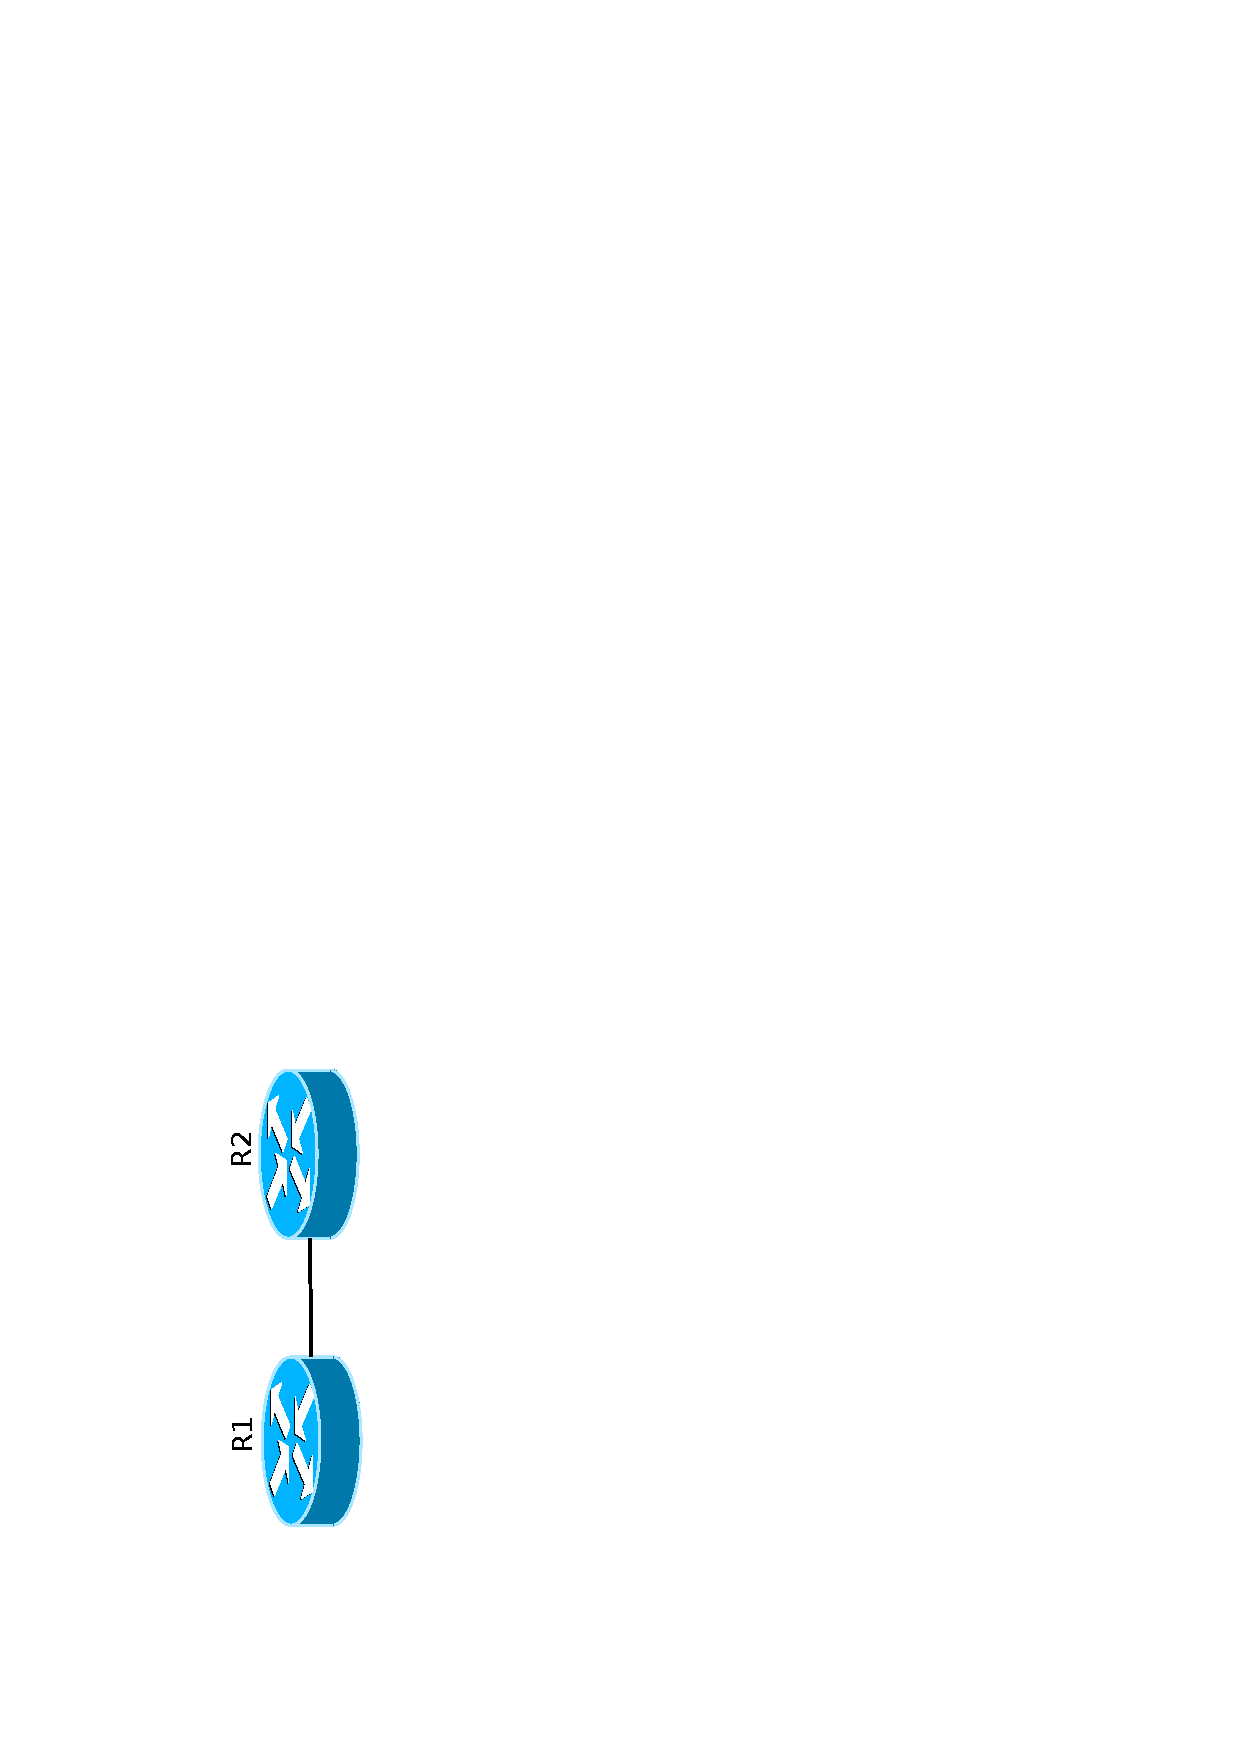
\includegraphics[height=0.3\textwidth, angle=-90, trim=100 50 420 500, clip]{../resultados/diagramaRed_Simple.pdf}
\end{center}
Supongamos que R1 se alcanza con TTL=$(i-1)$ y R2 con TTL=$i$. Además supongamos el siguiente comportamiento:
\begin{description}
 \item[R1] Tiene más prioridad en la cola de forwarding de paquetes (incluso podría tener distintas colas de prioridad según el campo
 {\tt ToS} del header IP) y una prioridad mucho menor en la cola de paquetes de tipo {\tt TIME-EXC}.
 \item[R2] Cumple alguna de las siguientes propiedades:
 \begin{itemize}
  \item No distingue prioridades.
  \item Distingue prioridades y tiene mayor prioridad sobre {\tt TIME-EXC}.
  \item Se comporta como R1, pero las colas de mayor prioridad tienen poca carga.
 \end{itemize}
\end{description}
Entonces si medimos $RTT^{acum}_{i-1}$ vamos a tener por un lado
el tiempo necesario para llegar a R1 y volver de R1 (que por simplicidad suponemos que es el mismo tiempo $t_{[0..i-1]}$) y por otro tendremos
el tiempo de encolamiento en R1 $q_{(i-1)}$.
$$ RTT^{acum}_{i-1} = 2t_{[0..i-1]} + q_{(i-1)}$$
En cambio si medimos $RTT^{acum}_i$, vamos a tener por un lado el tiempo $t_{[0..i-1]}$ de ida y vuelta, el tiempo del enlace entre R1 y R2
($t_{[i-1..i]}$) y el tiempo de encolamiento en R2 $q_{i}$.
$$ RTT^{acum}_{i} = 2t_{[0..i-1]} + 2t_{[i-1..i]} + q_{i}$$
Por las características de R1 y R2, sucederá que $q_{i} << q_{(i-1)}$ y si el delay en el enlace entre R1 y R2 es despreciable, tenemos que:
$$ RTT^{acum}_{i} < RTT^{acum}_{i-1}$$
Este comportamiento
es muy común en la práctica (ver Secciones \ref{resultados:cambridge}, \ref{resultados:ucrania}, \ref{resultados:china}). En particular
el comportamiento de R1 es muy común en Internet \cite{peterson}.






\subsection{Identificación de Enlaces Submarinos}
Hasta ahora analizamos cómo buscar las posibles rutas, luego identificamos una de ellas como la ruta más probable (o más ``pesada'') y en base
a esa calculamos el $RTT_i$ de cada salto. Ahora quisiéramos comparar entre sí esos valores para identificar el o los enlaces submarinos que
atravesamos en la ruta.

Para lograrlo utilizaremos el valor estándar de cada salto:
$$ ZRTT_i = \frac{RTT_i - \overline{RTT}}{SRTT}$$
donde $\overline{RTT}$ es el promedio y $SRTT$ el desvío estándar (con la corrección de Bessel):
$$ \overline{RTT} = \frac{1}{M} \sum_{i=1}^{M} RTT_i $$
$$ SRTT = \sqrt{\frac{1}{M-1}\sum_{i=1}^{M} (RTT_i - \overline{RTT})^2}$$
$M$ es la cantidad de saltos necesarios para llegar al host destino en la ruta más ``pesada''.

Estos valores normalizan la distribución de las variables $RTT_i$, de tal manera que:
\begin{itemize}
 \item Si $ZRTT_i > 0$, entonces está por encima de $\overline{RTT}$, es decir por encima de la media. Valores muy superiores al $RTT$ promedio
 pueden ser indicadores de saltos submarinos (o al menos un salto significativo).
 \item Al dividir por el desvío estándar se eliminan las distancias y se normalizan los valores, para que un mismo valor de $ZRTT_i$ en
 cualquier muestra tenga aproximadamente el mismo significado. Es decir que el valor estándar no dependerá de cada caso particular sino que tendrá
 un valor más general. Esto permitirá luego establecer un umbral genérico para identificar saltos submarinos.
\end{itemize}

La idea entonces será calcular estos valores y compararlos con los $RTT_i$ acumulados por cada salto (acumulado $k$-ésimo = $\sum_{i=1}^{k}RTT_i$)
y con los $RTT^{acum}_i$ (promedios de las mediciones originales).
Usamos ambos RTTs acumulados porque por la manera en que calculamos $RTT_i$ perdimos información de algunos saltos donde el RTT era negativo.
Si $ZRTT_i$ es grande y la acumulación de $RTT_i$s aumenta considerablemente, es esperable que allí encontremos un enlace submarino.

Una vez realizada la comparación, buscaremos un intervalo $I_u$ para cada uno de los casos de estudio, tal que dentro de ese intervalo podamos
asegurar que encontramos un enlace submarino (utilizando también la geolocalización de los nodos, ver Sección \ref{desarrollo:geolocalizacion}).
Luego, calcularemos la interseccion de esos intervalos y trataremos de establecer un umbral genérico que suponemos tendrá sentido en casos de
estudio futuros.
%% buscar un umbral aproximado que sirva en los 3 casos de estudio de ser posible (en esta seccion solo contamos la idea y como la vamos a experimentar)

%% grafico zscores vs rtt_i acumulados






\subsection{Geolocalización de Rutas} \label{desarrollo:geolocalizacion}
%% herramientas de geolocalizacion. Explicacion de mapas a crear
Aparte del análisis numérico que realizamos en las secciones previas, vamos a intentar ubicar en un mapa a cada uno de los saltos intermedios.

El análisis consistirá de la geolocalización de la ruta de mayor probabilidad que mencionamos en secciones anteriores. Para esto utilizaremos
servicios de geolocalización \cite{geolocation} que por cada IP nos indicarán donde fue registrada la red a la que pertenece. De esta manera
podremos conocer la ubicación del router. Debemos dejar en claro que podría suceder que una red estuviera registrada en un país pero que algunos
nodos conectados a esa red estén en otros países. En un caso así, claramente tendríamos una respuesta errónea por parte de esos servicios. Tomaremos
algunas medidas para evitarlo.

Como ya fue mencionado en la Sección \ref{desarrollo:rutas}, el nodo que responde lo hace usando la IP correspondiente a la interfaz por la cual
recibió nuestro paquete. Veamos un ejemplo:

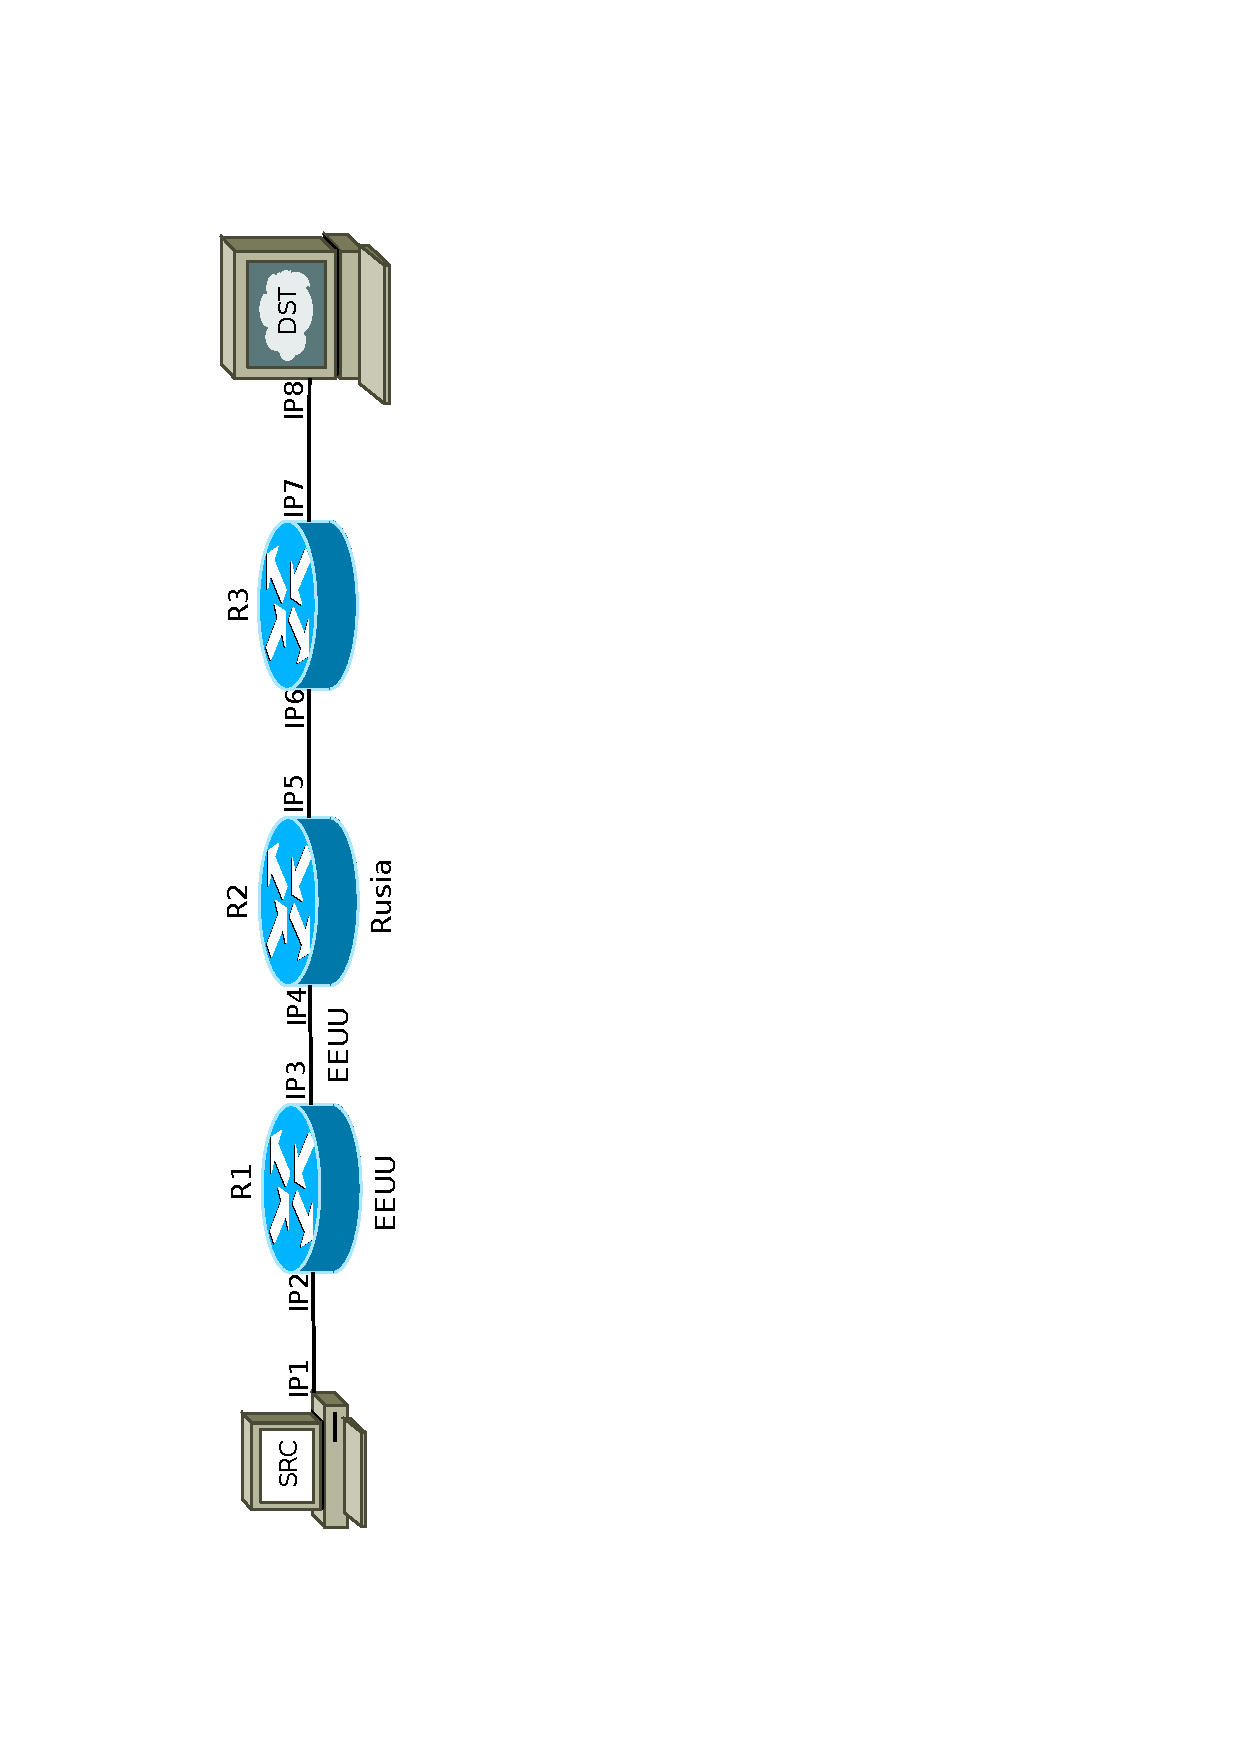
\includegraphics[height=\textwidth, angle=-90, trim=100 50 380 50]{../resultados/diagramaRed.pdf}

R2 está ubicado en Estados Unidos y R3 en Rusia. El enlace R2-R3 es una red cuya dirección fue registrada en Estados Unidos, con lo cual
en los registros internacionales, tanto IP3 como IP4 se encuentran en Estados Unidos.

Si R2 nos envía un paquete time-exceeded, la IP fuente del paquete será IP4. Cuando geolocalicemos IP4, encontraremos que su ubicación es
Estados Unidos. Pero R2 pertenecía a Rusia, ¿cómo podríamos saberlo?.

Para solucionar este problema, utilizaremos los RTTs calculados en secciones previas:
\begin{itemize}
 \item Si el RTT del salto es pequeño, se considera que R2 pertenece a Estados Unidos.
 \item Si el RTT del salto es grande, en cambio, lo que haremos es mirar el siguiente salto. Cuando R3 responda time-exceeded,
lo hará usando IP6. Es muy probable que R3 también se encuentre cerca de R2 (en Rusia tal vez), pero de todas formas nosotros
\emph{asumiremos} que R2 se encuentra en el país donde fue registrada la red R2-R3.
\end{itemize}

En el ejemplo, el RTT del salto debería ser grande y entonces usaríamos el segundo caso.

Esta heurística es una aproximación de la realidad, claramente no es ciento porciento eficaz.
En casos donde haya ambigüedades o que esta heurística no funcione, utilizaremos otra manera de determinar la ubicación real: El \emph{DNS (Domain Name
System)}. La idea es usar reverse DNS para obtener el nombre de cada IP. Dado que los nombres están destinados a la lectura de seres humanos, esperamos
encontrar allí pistas que nos permitan deducir dónde estamos, o al menos si hubo o no hubo algún salto importante. Para esto utilizaremos el módulo
{\tt socket} de Python.

Nuevamente debemos aclarar que el nombre del dominio podría estar desactualizado o bien podríamos equivocarnos al realizar deducciones sobre el mismo,
con lo cual tampoco es una heurística del todo eficaz.

En conclusión, por cada IP del camino más ``pesado'', determinaremos la ubicación geográfica en base a:
\begin{itemize}
 \item $RTT_i$ y $ZRTT_i$ del salto.
 \item Geolocalización del servicio web (país, ciudad, coordenadas).
 \item DNS.
\end{itemize}

La idea es que luego de haber geolocalizado a todas las IPs (o conjuntos de IPs si hay muchas en una misma región), vamos a medir la distancia
recorrida en cada salto, utilizando la herramienta de Google Maps\cite{googlemaps}. Esta distancia será comparada con los RTTs acumulados de algunos saltos
(en los que sea posible realizar la comparación) y luego buscaremos una relación entre todos los casos de estudio.
Utilizaremos RTTs acumulados ($RTT^{acum}_i$) porque es la medición de RTT menos sesgada que tenemos (dado que al calcular
$RTT_i$ algunos valores quedan en cero).
%% Lo logico es que la realación sea nula, porque en realidad va a pasar que no depende solo de la distancia el RTT, sino tmb 
%% del tiempo de encolamiento.

Por otro lado, la geolocalización en un mapa nos permitirá encontrar de una manera visual los enlaces submarinos.


\subsection{Casos de Estudio}
Se analizarán las siguientes rutas:
\begin{description}
 \item[Cambridge:] La ruta tendrá como destino la Universidad de Cambridge (\url{www.cam.ac.uk}, IP: {\tt 131.111.150.25}). Se encuentra en
 Cambridge, Inglaterra. El origen será un host ubicado en Lanús (Provincia de Buenos Aires), utilizando el proveedor de servicios de internet
 ``Telecentro''.
 
 \item[Ucrania:] La universidad que elegimos como destino es National Taras Shevchenko University of Kyiv (\url{www.univ.kiev.ua}, IP: {\tt 91.202.128.77 
}). Esta se encuentra en Kiev, Ucrania. El host origen se ubica en Lanús (Provincia de Buenos Aires), utilizando el proveedor de servicios de internet
 ``Telecentro''.
 
 \item[China:] La universidad que elegimos como destino es The Chinese University of Hong Kong (\url{www.cuhk.edu.hk}, IP: {\tt 137.189.11.73 }).
 Esta se encuentra en Hong Kong, China. El host origen se ubica en Lanús (Provincia de Buenos Aires), utilizando el proveedor de servicios de internet
 ``Telecentro''.
 
 
\end{description}